\section*{Introduction} % Pas de numérotation
\addcontentsline{toc}{section}{Introduction} % Ajout dans la table des matières

Dans le cadre de notre cours d'algorithmique avancée nous avons été amenés à réaliser un algorithme de notre choix parmi une liste de projet proposée. J'ai, a mon plus grand regret, trouvé l'idée de faire le chemin le plus cours avec l'algorithme de Dijkstra avec deux graphe amusante. L'un avec une structure en vecteur et l'autre avec une structure en brin. Le graphe quand à lui represente le metro de berlin.

L'intitulé exacte est :
\smallbreak
\fbox{\parbox{\linewidth-2\fboxrule-2\fboxsep}{
		Gérer un réseau de transports en commun, par exemple le métro de Berlin, via un graphe (Vec et Brin). Résoudre dans ce cas le problème du plus court chemin, algorithme de Dijkstra.
}}

\begin{figure}[h]
\centerline{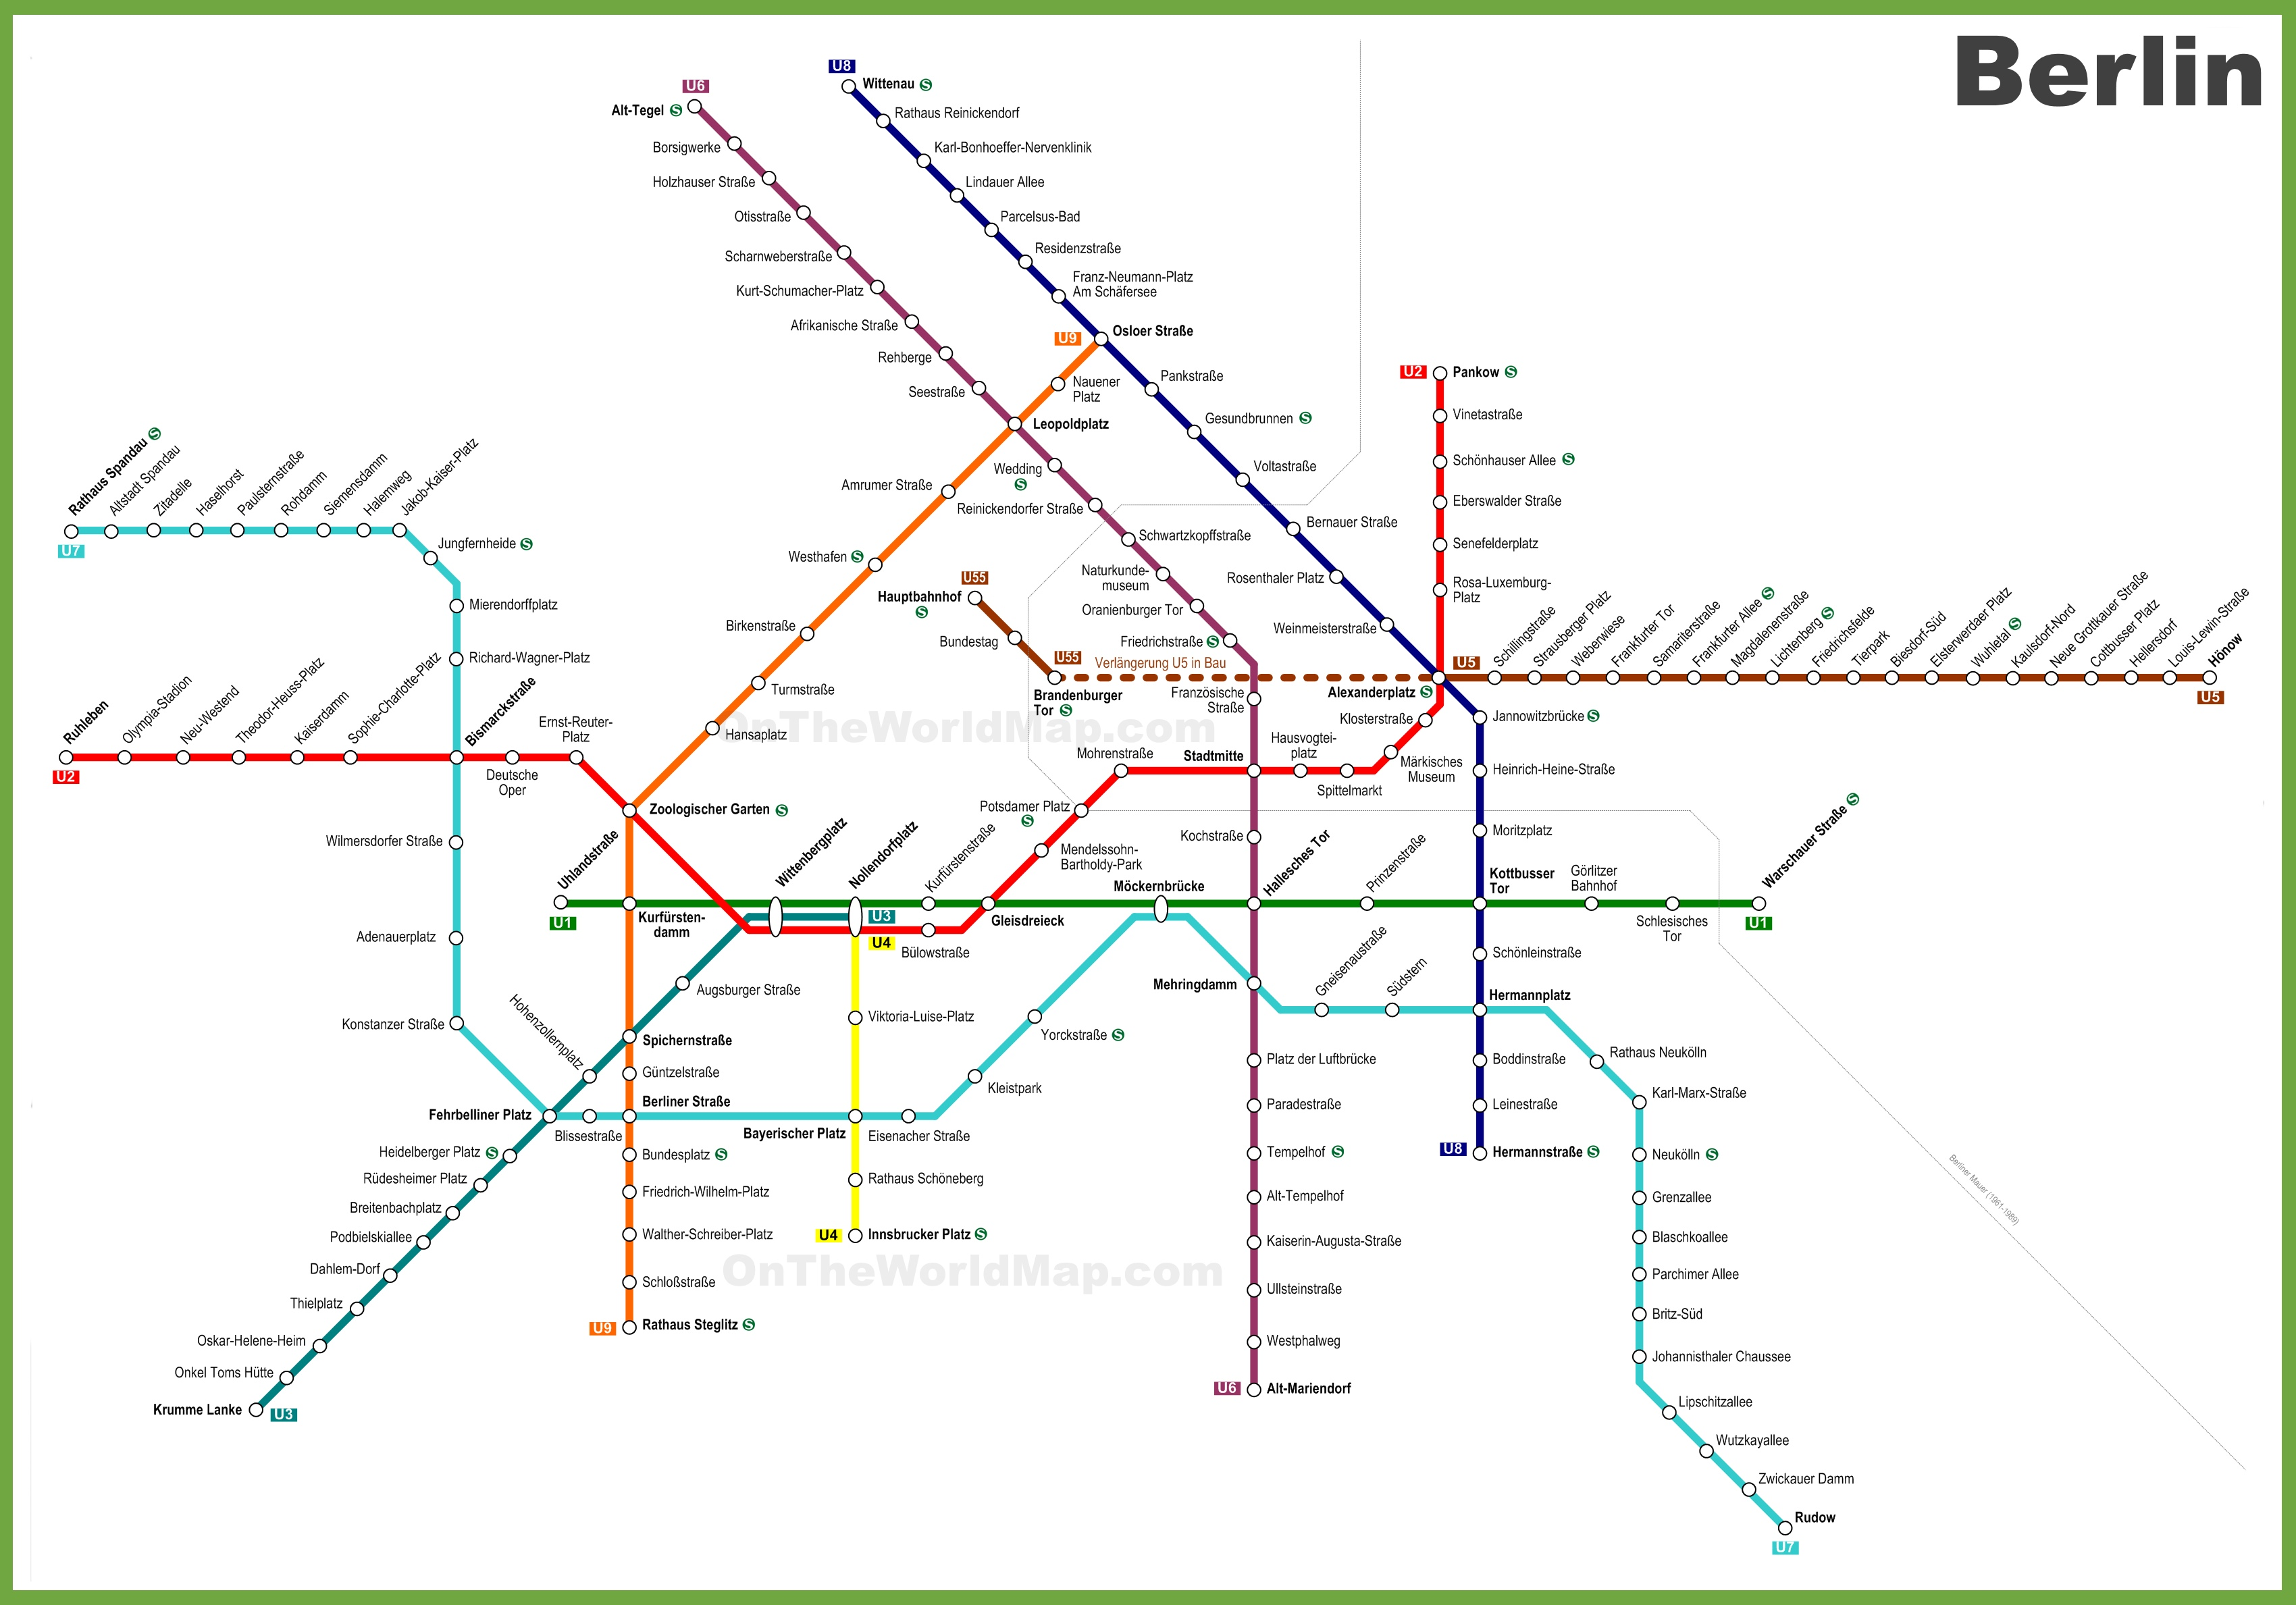
\includegraphics[width=1\textwidth]{images/metro.jpg}}
\caption{\label{legende} Metro de berlin.
}
\end{figure}

\smallbreak

Le métro de Berlin, inauguré en 1902, est composé de 173 station étendu sur 146,3 km. Il est consideré comme un très beau métro.

